\begin{frame}{A Taxonomy of Repeated Games Models}
    \begin{figure}
        \tikzstyle{mybox} = [draw=gray!20, fill=white, very thick,
        rectangle, rounded corners, inner sep=10pt, inner ysep=10pt]
        \tikzstyle{fancytitle} = [fill=gray, text=white, rounded corners]
        \scalebox{0.7}{
        \begin{tikzpicture}
            \node [mybox] at (0, 0) (gen-mod){%
                \begin{minipage}{0.50\textwidth}
                    \vspace{-0.25cm}
                    \[ \Gamma^r = (N, \Theta, (D_i, S_i, u_i)_{i\in N}, q, p) \]
                \end{minipage}
            };
            \node [inner sep=0pt] (gen-mod-img) at (-4.4, 0.5){%
                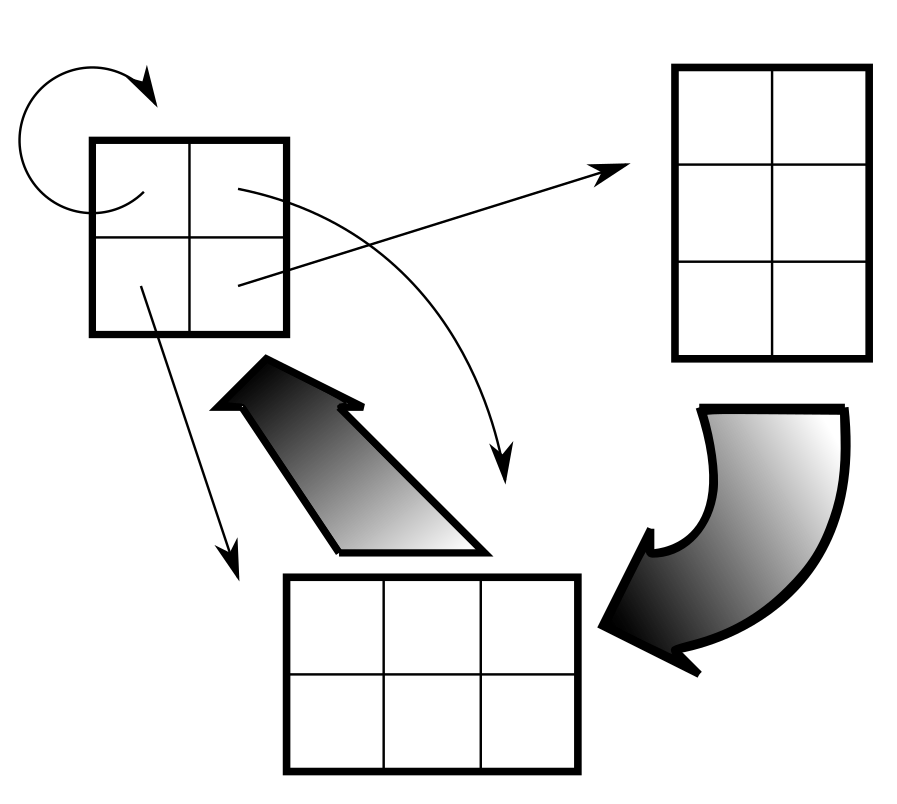
\includegraphics[width=0.25\textwidth]{img/stochastic.png}
            };
            
            \node [mybox] at (-4.5, -3) (mdp){%
                \begin{minipage}{0.40\textwidth}
                    {\color{green}Single-agent stochastic game}
                    \vspace{-0.25cm}
                    \[ |N| = 1. \]
                \end{minipage}
            };
            
            \node [mybox] at (0, -7.5) (state){%
                \begin{minipage}{\textwidth}
                    {\color{green}At every round, every player knows the
                    current state of nature $\theta \in \Theta$.} \\
                    Informally, for each player $i \in N$, there exists some
                    state $w(s_i) \in \Theta$ such that the signal $s_i$ can
                    never occur unless the current state is $w(s_i)$.
                \end{minipage}
            };
            
            \node [mybox, draw=black] at (4.5, -3.5) (std){%
                \begin{minipage}{0.60\textwidth}
                    \begin{itemize}
                        \item {\color{green}Only one possible state of
                        nature}
                        \[ |\Theta| = 1. \]
                        \item {\color{green}Players know all of each other's past
                        moves}
                        \[ S_i = \bigtimes_{j\in N-i} D_j. \]
                    \end{itemize}
                \end{minipage}
            };
            \node [inner sep=0pt] (gen-mod-img) at (7, -5.5){%
                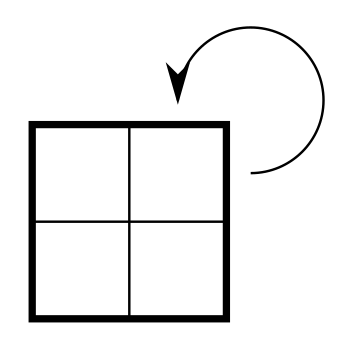
\includegraphics[width=0.20\textwidth]{img/std.png}
            };

            \node[fancytitle] at (gen-mod.north) {Stochastic Games (General Model)};
            \node[fancytitle] at (mdp.north) (mdp-title) {Markov Decision Processes};
            \node[fancytitle] at (state.north) (state-title) {Complete State Information};
            \node[fancytitle, fill=black] at (std.north) (std-title) {Standard Repeated Games};

            \draw[thick, -Latex] (gen-mod.west) -- (mdp-title.north);
            \draw[thick, -Latex] (gen-mod.south) -- (state-title.north);
            \draw[thick, -Latex] (gen-mod.east) -- (std-title.north);
        \end{tikzpicture}}
        \caption{A taxonomy of repeated game models.}
    \end{figure}
\end{frame}

\begin{frame}{Repeated game with standard information}
    \metroset{block=fill}
    \begin{block}{Definition}
        A \textbf{standard repeated game} is a repeated game in which there is only one state of
        possible state of nature
		$$|\Theta| = 1,$$
        the players know all of each other's past moves
        $$S_i = \bigtimes_{j \in N} D_j \quad \forall i$$
        and
		$$p(d,...,d,\theta | d, \theta) = 1 \quad \forall d \in D.$$
    \end{block}
\end{frame}


\begin{frame}{Example : the game of Chicken}
    \begin{exampleblock}{Example}
        Consider the game of Chicken in normal form
        \begin{table}
            \begin{tabular}{c|cc}
                & {\color{red}$a_2$}    & {\color{red}$b_2$} \\
                \hline
                {\color{green}$a_1$}    & \payoff{4}{4}   & \payoff{1}{6} \\
                {\color{green}$b_1$}    & \payoff{6}{1}    & \payoff{-3}{-3} 
            \end{tabular}
            \caption{Game of Chicken in normal form}
        \end{table}
    
    \end{exampleblock}
    \note{
		Draw the normal form on the board    
		
		Explain the anecdote
    }
\end{frame}

\begin{frame}{Equilibrium of the game}
\textbf{Equilibrium analysis}

\begin{itemize}
	\pause
	\item Single shot case
	\begin{itemize}
		\item Pure strategie : Nash equilibrium : $(1,6) \quad (6,1)$
		\item Randomized equilibrium : $u_i = 0.5\cdot4 + 0.5 \cdot (6+1-3) = 3$
		\item Correlated equilibrium : $u_i = 0.5\cdot4 + 0.25 \cdot (6+1) =  3.75$
	\end{itemize}
	\pause
	\item Repetition of the game with standard information $$u_i = ??$$
\end{itemize}
	\pause
	Tit-for-tat is an equilibrium if $\delta \geq \frac{2}{3}$
\end{frame}

\note{
	Say that $(a_1,a_2)$ is not an sub-game perfect of the \textbf{one round} game because both players would want to play $b$

	\begin{itemize}
		\item \textbf{HYP}
			\begin{itemize}
				\item Infinitely repeated game with standard information
				\item Player 1 choose a $\delta$ between 0 and 1, what value of $\delta$
				\item Player 2 begin to be bold, and then be cautious at every round
			\end{itemize}
		\item Compute the $\delta$-discounted average payoff : $(1-\delta)(6+1\delta+\sum_{k=3}^\infty 4\delta^{k-1} ) = 6 - 5\delta + 3 \delta^2$
		\item $\delta$-discounted average if no deviation from tit-for-tat : $4 \geq 6 - 5\delta + 3 \delta^2$
		\item Tit-for-Tat is an equilibrium if $\delta \geq \frac{2}{3}$
	\end{itemize}
}

\begin{frame}{Going further with the Tit-for-Tat strategy in a standard information game}
	
	\textbf{Going further}
	\begin{itemize}
	\item What will be the $\delta$-discounted average payoff if both player decide to play Tit-for-Tat after player 2 deviation ?
	\pause
	
	\item What will be the $\delta$-discounted average payoff if p1 deviates from Tit-for-Tat after player 2 deviation. Then both play Tit-for-Tat.
	\pause
	\item What $\delta$ should we choose so that neither player can gain by being the first to deviate ?
	\end{itemize}
	\note{
	\textbf{Going further}
	\begin{itemize}
		\item If both player play Tit-for-tat after P2 deviation $(1-\delta)(1+6\delta+1\delta^2+6\delta^3+...) = \frac{1+6\delta}{1+\delta}$
		\item If P1 deviate after P2 deviation $(1-\delta)(1+4\delta+4\delta^2+4\delta^3+...) = 1+3\delta$
		\item $1+3\delta > \frac{1+6\delta}{1+\delta}$ when $\delta > \frac{2}{3}$
	\end{itemize}
	
	\textbf{Grim strategy}
	
	Only explain that such unforgiving punishment is not rational and extreme. We might be interested in finding other strategies.			
	}
\end{frame}

\begin{frame}{Finding mutual punishment strategies}
	\metroset{block=fill}
    \begin{block}{Mutual punishment strategy}
        For a player i, a {\color{green}mutual punishment strategy} can be :
        \begin{itemize}
        	\item On the first round : i plays $a_i$ \pause
        	\item If last round was $(a_1,a_2) \text{ or } (b_1,b_2)$, i plays $a_i$ \pause
        	\item If last round was $(a_1,b_2) \text{ or } (b_1,a_2)$, i plays $b_i$
        \end{itemize}
    \end{block}
    \textbf{\color{green}Interpretation}
    
    If both players follow the strategy, their expected payoff is 4. If one deviate, the other punish him until he participate himself in his own punishment.
    
    \textbf{\color{green}Is it a sub-game perfect equilibrium to follow the mutual punishment strategy?}
    
    \note{
		\textbf{If strategy call for $b_i$ but play $a_i$}
		
		Deviation is noob if $4+4\delta \geq 6 - 3 \delta \qquad \Rightarrow \delta \geq \frac{2}{7}$ not worth to deviate
		
		\textbf{If strategy call for $a_i$ but play $b_i$}
		
		Deviation is noob if $-3+4\delta \geq 1 - 3\delta \qquad \Rightarrow \delta	\geq \frac{4}{7}$ not worth to deviate
		
		    
    }
\end{frame}

\begin{frame}{Take home message \#6}
    \metroset{block=fill}

    \begin{block}{Take-home-message \#6}
        \vspace{0.2cm}
        \begin{columns}
            \begin{column}{0.65\textwidth}
                A \textbf{repeated game with standard information} is a repeated game where
                \begin{itemize}
                    \item there is {\color{green}only one possible state of nature}
                    \item the players {\color{green}know all of each other's past moves}
                \end{itemize}
            \end{column}
            \begin{column}{0.2\textwidth}
                \begin{center}
                    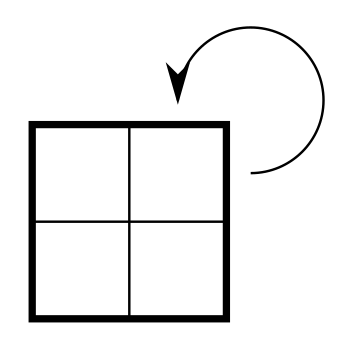
\includegraphics[width=0.7\linewidth]{img/std.png}
                \end{center}
            \end{column}
        \end{columns}

        \vspace{0.5cm}
        Depending on the value of the discount factor $\delta$, several strategies might constitute
        an equilibrium: \textit{tit-for-tat}, \textit{getting-even}, \textit{grim}, etc.
        However, these equilibria might not always be subgame perfect.
    \end{block}
\end{frame}
